\chapter{Introduction}
\label{intro}
	
I'll give you some samples here to get you started.\par

Example 1: List your ideas by \textbf{itemize}. 
\begin{itemize}
	\item Step 1: The serving eNB informs the UE in which event the received signal strength should be reported through a configuration message, and the UE keeps track of the received signal strength of its serving cell and neighboring cells.
	\item Step 2: Upon a specified event\footnote{Further details can be found in~\cite{ts36.331}.} happens, the UE sends measurement reports to the eNB.
	\item Step 3: The serving eNB decides whether to initiate a handover (HO) procedure to the selected target cell based on the information received from the UE measurement reports and the status of the neighboring cells.
\end{itemize}



EXample 2: Insert figures using \textbf{figure}. See Figure~\ref{fig:HandoverSpec}.
	
\begin{figure}[t]
	\vspace{-3mm}
	\graphicspath{ {../Figures/} } 
	\centering 
	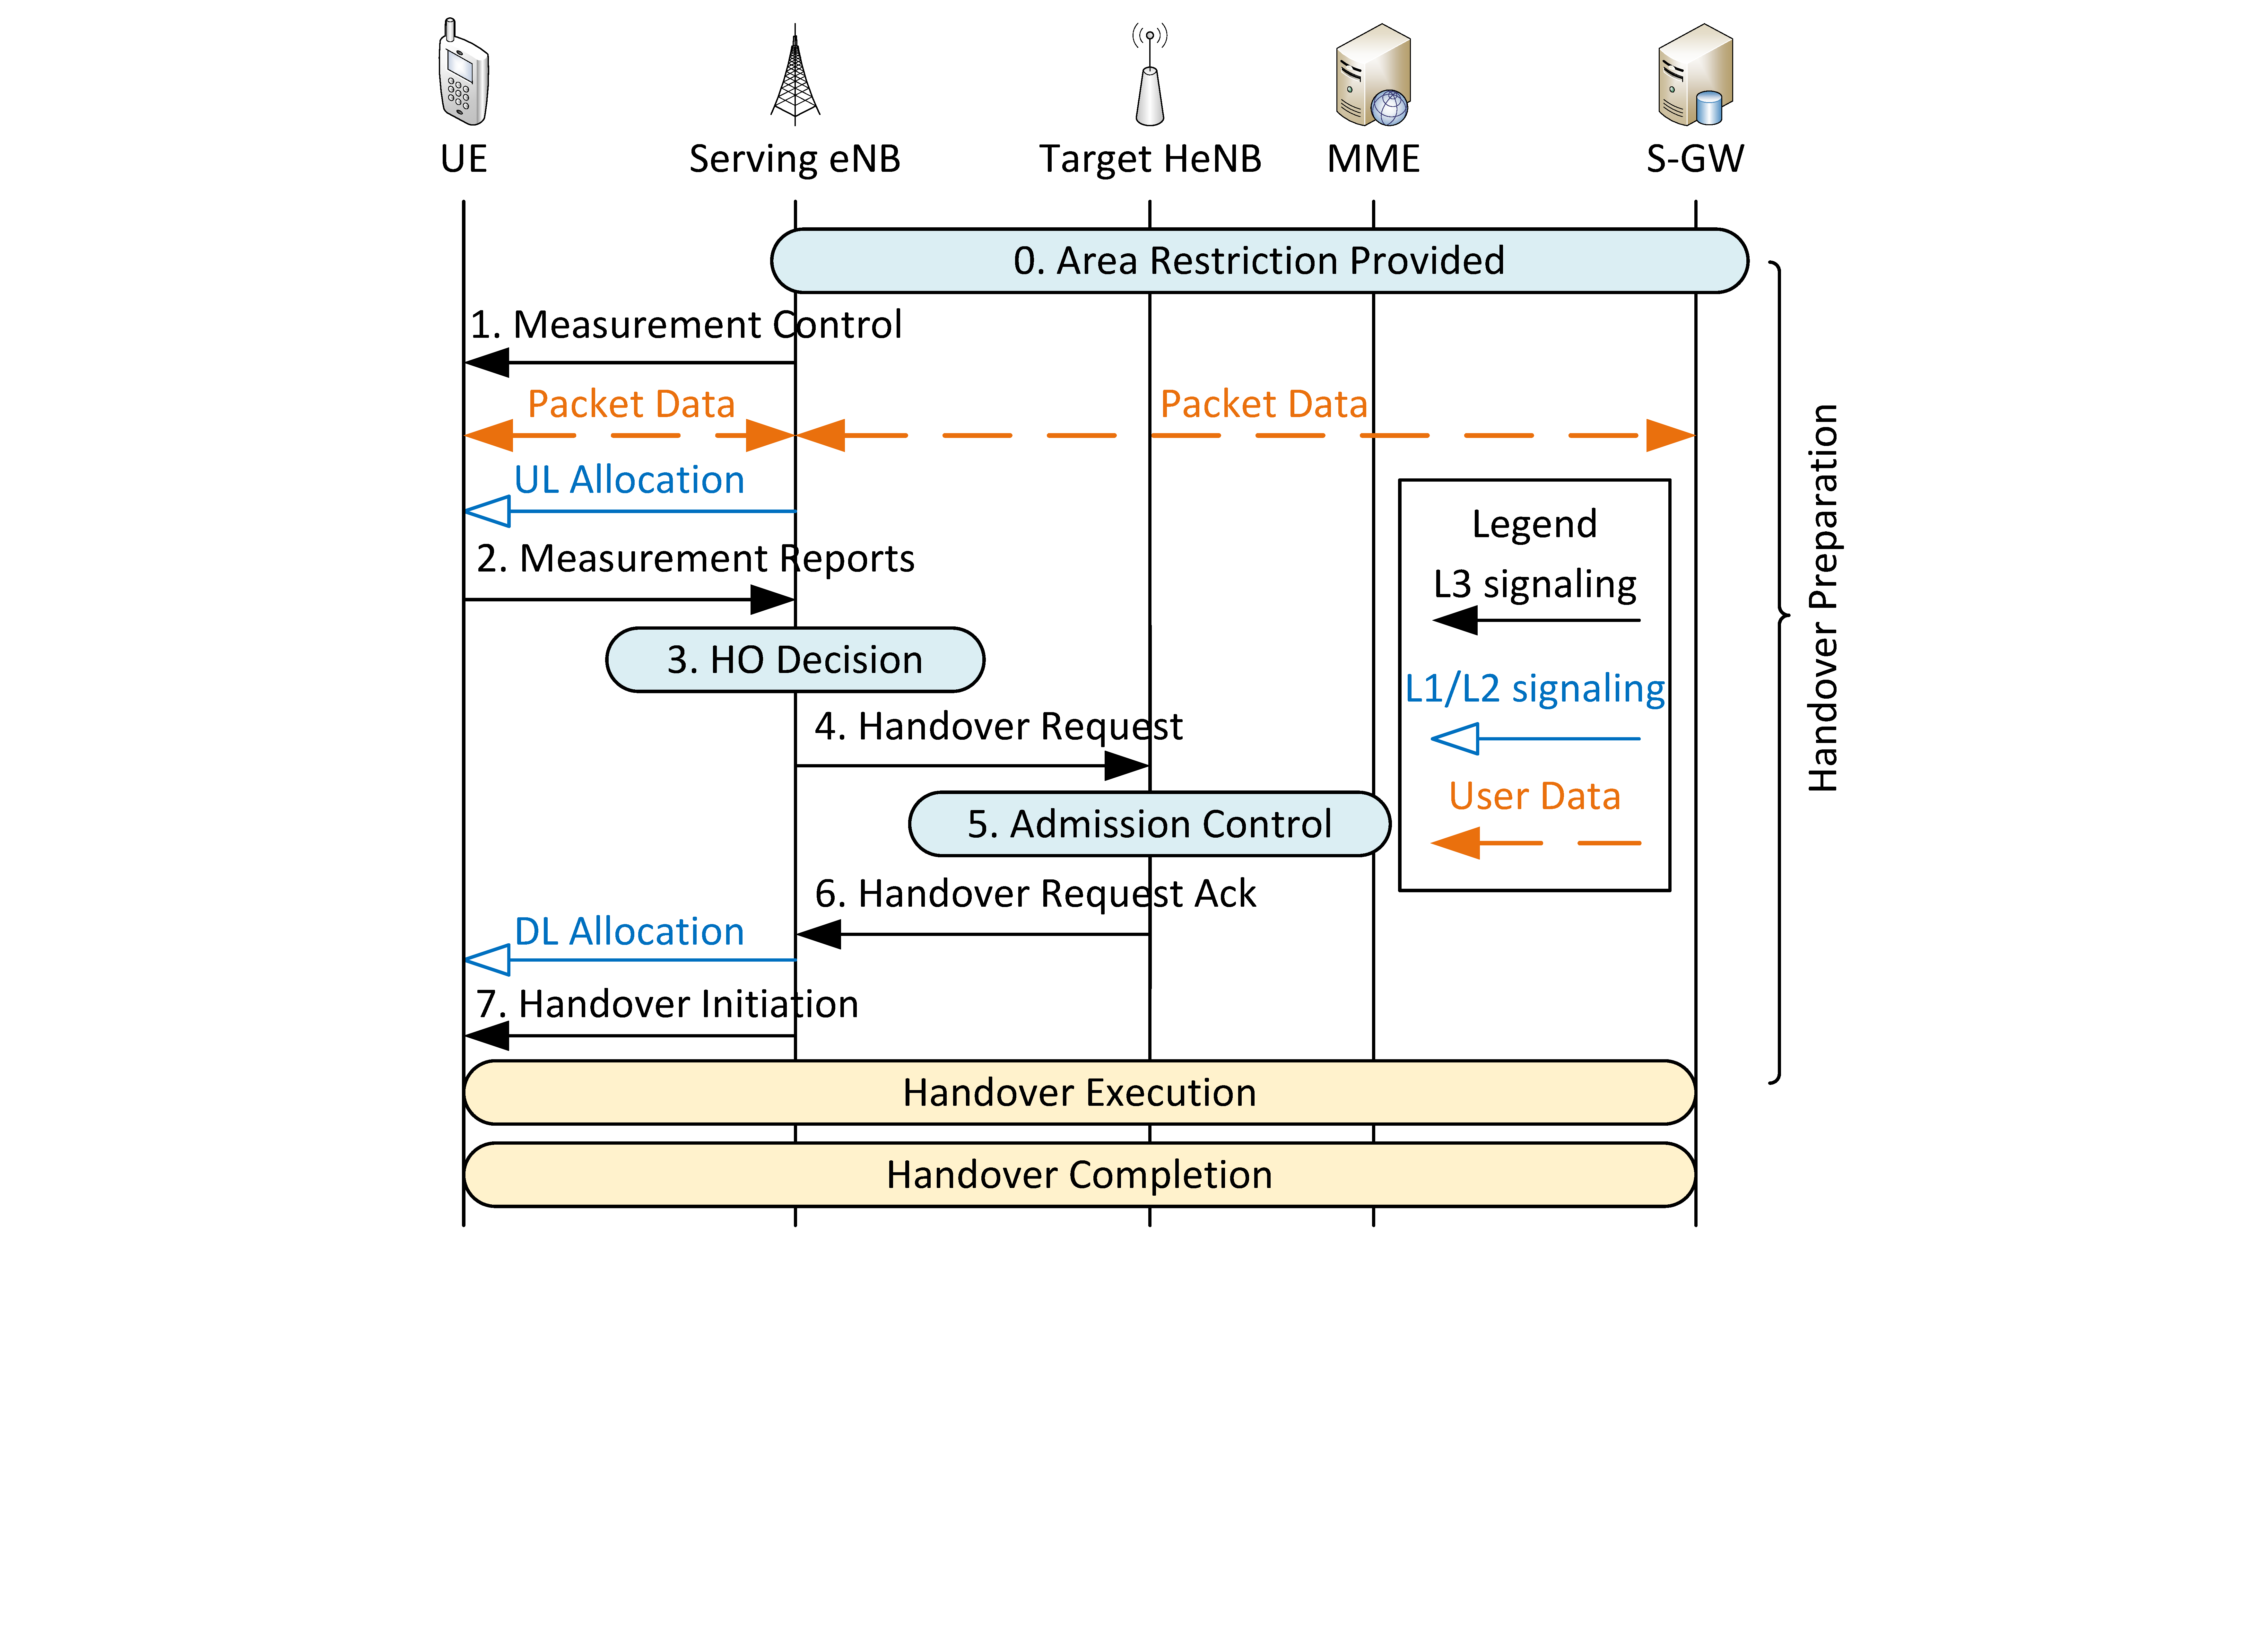
\includegraphics[width=8cm]{handover_spec.pdf} 
	\caption{Handover procedure specified in the 3GPP standard.} 
	\label{fig:HandoverSpec} 
	\vspace{-5mm}
\end{figure}

Example 3: Insert tables using \textbf{tabular}. See Tables~\ref{tab:ParameterSetting}.

\begin{table}[t]
	\caption{List of Parameters}
	\centering  
	\label{tab:ParameterSetting}		
	\begin{tabular}{| p{6.5cm}|c|}
		\hline
		                                                          & \textbf{Parameter} \\ \hline\hline
		Probability density function of $t_s$                     &      $f_s(t)$      \\ \hline
		Probability density function of $t_{f}$                   &     $f_{f}(t)$     \\ \hline
		Probability density function of $t_{m}$                   &     $f_{m}(t)$     \\ \hline
		Probability density function of $t_{o}$                   &     $f_{o}(t)$     \\ \hline
	\end{tabular}
\end{table}

Example 4: Write equations using \textbf{equation}.
      
\begin{equation}
	E[N_{t}(t_{o}) | \text{Case1-1} ] =
	\frac{ \eta_{m}f^{*}_{f}(\eta_{s})[1-f^{*}_{m}(\eta_{s})]^{2} (1+\alpha) } 
	{ \eta_{s} (1- f^{*}_{m}(\eta_{s})f^{*}_{f}(\eta_{s}))^{2} } \ .
\end{equation}


\chapter{Background}
\label{sec:Background}
Write your own content...
	
\chapter{Related Work}
\label{relatedwork}
Write your own content...	

\chapter{Proposed Scheme}
\label{proposedscheme}
Write your own content...

\chapter{Analytical Model}
\label{analyticalmodel}
Write your own content...	

\chapter{Simulation and Numerical Results}
\label{simulationandnumericalresults}
Write your own content...
	
\chapter{Conclusions}
\label{conclusion}
Write your own content...
	
\chapter{Furture Work}
Write your own content...





